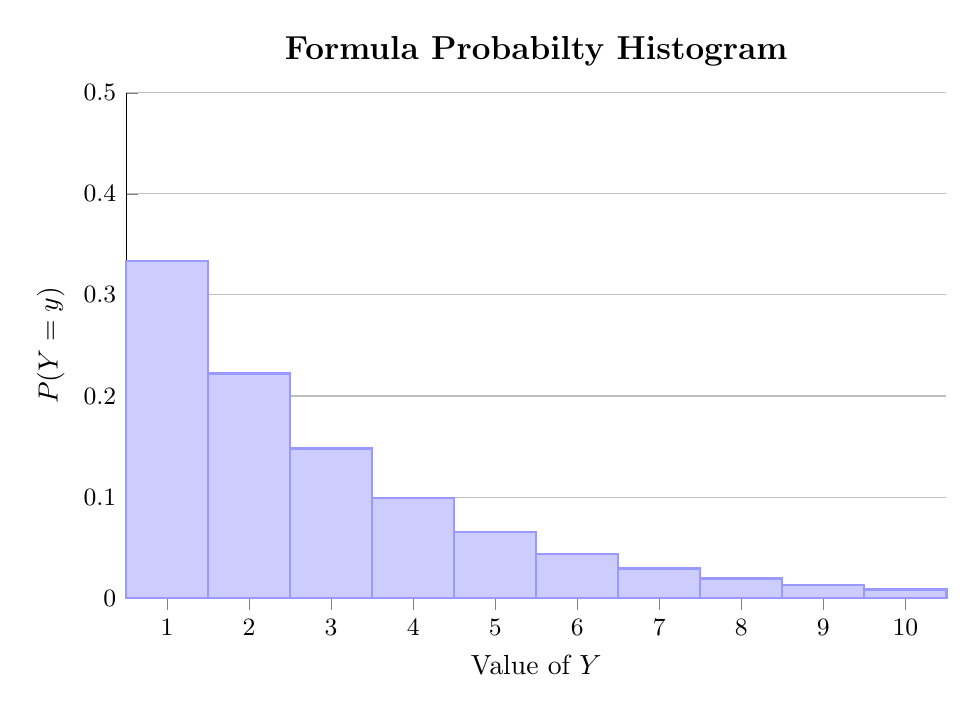
\begin{tikzpicture}
  \begin{axis}[
      axis lines*=left,
      no markers,
      samples at={1,2,...,10},
      xmin=0.5, xmax=10.5, ymin=0, ymax=0.5,
      xtick={0,1,...,10},
      ytick={0,0.1,0.2,0.3,0.4,0.5},
      xlabel={Value of $Y$},
      ylabel={$P(Y=y)$},
      title={\large\bf Formula Probabilty Histogram},
      ticklabel style={font=\small},
      enlargelimits=false,
      clip=false,
      grid = none,
      ymajorgrids=true,
      ybar=0pt,
      bar width=1,
      width=12cm,
      height=8cm
    ]
    \addplot+[thick,fill=blue!20,draw=blue!40]  { (1/3)*(2/3)^(x-1) };
  \end{axis}
\end{tikzpicture}
